%%%%%%%%%%%%%%%%%%%%%%%%%%%%%%%%%%%%%%%%%%%%%%%%%%%%%%%%%%%%%%%%%%%%%%%
%%%%%%%%%%%%%%%%%%%%%%%%%%%%%%%%%%%%%%%%%%%%%%%%%%%%%%%%%%%%%%%%%%%%%%%
%%%%%                                                                 %
%%%%%     <file_name>.tex                                             %
%%%%%                                                                 %
%%%%% Author:      Renzo Andri                                        %
%%%%% Created:     21.12.2013                                         %
%%%%% Description: Chapter about Design Implementations and           %
%%%%%              Performance Data.                                  %
%%%%%                                                                 %
%%%%%%%%%%%%%%%%%%%%%%%%%%%%%%%%%%%%%%%%%%%%%%%%%%%%%%%%%%%%%%%%%%%%%%%
%%%%%%%%%%%%%%%%%%%%%%%%%%%%%%%%%%%%%%%%%%%%%%%%%%%%%%%%%%%%%%%%%%%%%%%


\chapter{Design Implementation}
\textit{This chapter is about the architecture variant you actually
implemented and its resulting performance; e.g., SNR, image quality,
peak throughput, required bandwidth ... (whatever quality and
performance metrics apply). In an ASIC or FPGA project you would also
specify the key figures of your design; e.g., area/lut usage, timing
figures, interface widths... In an ASIC project you would also talk
about backend specific things such as the floorplan of your chip,
design for test (and test coverage), power simulation, special
clocking circuitry and pad/bonding diagrams.}


\section{Instruction Table}
The following Table \ref{tab:instr} gives an overview of the implementented \gls{orbis} instructions. See Table \ref{tab:instr_det} for more detailled information about the functionality of each instruction and consider Table \ref{tab:conv} for naming conventions.
%\begin{landscape}
\begin{longtable}{|p{1.8cm}|l|p{10cm}|}
\caption[Instructions]{Instructions}

\label{tab:instr}
\endfirsthead
\multicolumn{3}{c}{Table \ref{tab:instr}: Instructions (contin.)} \\ \hline
Instruction & Parameter & Description \\ \hline
\endhead
\endfoot
\endlastfoot
\hline
Instruction & Parameter & Description \\ \hline
l.bf&N&Brach if Flag\\ \hline
l.bnf&N&Branch if not Flag\\ \hline
l.j&N&Jump Immediate\\ \hline
l.jal&N&Jump and Link\\ \hline \hline

l.nop&K&No Operation\\ \hline \hline

l.jalr&rB&Jump and Link Register\\ \hline
l.jr&rB&Jump Register\\ \hline \hline

l.movhi&rD, K&Move High\\ \hline
l.addi&rD, rA, I&Add Immediate\\ \hline
l.addic&rD, rA, I&Add Immediate Carry\\ \hline
l.andi&rD, rA, K&Bitwise And Immediate\\ \hline
l.lbs&rD, I(rA)&Load Byte Signed\\ \hline
l.lbz&rD, I(rA)&Load Byte Unsigned\\ \hline
l.lhs&rD, I(rA)&Load Halfword Signed\\ \hline
l.lhz&rD, I(rA)&Load Halfword Unsigned\\ \hline
l.lws&rD, I(rA)&Load Word Signed\\ \hline
l.lwz&rD, I(rA)&Load Word Unsigned\\ \hline
l.mfspr&rD, rA, K&Move from Special-Purpose Register\\ \hline
l.muli&rD, rA, I&Multiply Immediate\\ \hline
l.ori&rD, rA, K&Bitwise Or Immediate\\ \hline
l.xori&rD, rA, I&Bitwise Exclusive Or Immediate\\ \hline \hline

l.rori&rD, rA, L&Rotate Right Logic Immediate\\ \hline
l.slli&rD, rA, L&Shift Left Logic Immediate\\ \hline
l.srai&rD, rA, L&Shift Right Arithmetic Immediate\\ \hline
l.srli&rD, rA, L&Shift Right Logic Immediate\\ \hline \hline

l.mtspr&rA, rB, K&Move to Special-Purpose Register\\ \hline
l.sb&I(rA), rB&Store Byte\\ \hline
l.sh&I(rA), rB&Store Halfword\\ \hline
l.sw&I(rA), rB&Store Word\\ \hline \hline
 
l.add&rD, rA, rB&Add\\ \hline
l.addc&rD, rA, rB&Add Carry\\ \hline
l.and&rD, rA, rB&Bitwise And\\ \hline
l.or&rD, rA, rB&Bitwise Or\\ \hline
l.sll&rD, rA, rB&Shift Left Logic\\ \hline
l.sra&rD, rA, rB&Shift Right Arithmetic\\ \hline
l.srl&rD, rA, rB&Shift Right Logic\\ \hline
l.sub&rD, rA, rB&Subtract\\ \hline
l.xor&rD, rA, rB&Bitwise Exclusive Or\\ \hline
l.mul&rD, rA, rB&Multiply\\ \hline
l.mulu&rD, rA, rB&Multiply Unsigned\\ \hline
l.muld&rA, rB&Multiply Double-Word\\ \hline
l.muldu&rA, rB&Multiply Double-Word Unsigned\\ \hline \hline

l.sfeq&rA, rB&Set Flag if Equal\\ \hline
l.sfges&rA, rB&Set Flag if Greater Equal Signed\\  \hline
l.sfgeu&rA, rB&Set Flag if Greater Equal Unsigned\\ \hline
l.sfgts&rA, rB&Set Flag if Greater than Signed\\ \hline
l.sfgtu&rA, rB&Set Flag if Greater than Unsigned\\ \hline
l.sfles&rA, rB&Set Flag if Less Equal Signed\\ \hline
l.sfleu&rA, rB&Set Flag if Less Equal Unsigned\\ \hline
l.sflts&rA, rB&Set Flag if Less than Signed\\ \hline
l.sfltu&rA, rB&Set Flag if Less than Unsigned\\ \hline
l.sfne&rA, rB&Set Flag if not Equal\\ \hline \hline

l.sfeqi&rA, I&Set Flag if Equal Immediate\\ \hline
l.sfgesi&rA, I&Set Flag if Greater Equal Signed Immediate\\ \hline
l.sfgeui&rA, I&Set Flag if Greater Equal Unsigned Immediate\\ \hline
l.sfgtsi&rA, I&Set Flag if Greater than Signed Immediate\\ \hline
l.sfgtui&rA, I&Set Flag if Greater than Unsigned Immediate\\ \hline
l.sflesi&rA, I&Set Flag if Less Equal Signed Immediate\\ \hline
l.sfleui&rA, I&Set Flag if Less Equal Unsigned Immediate\\ \hline
l.sfltsi&rA, I&Set Flag if Less than Signed Immediate\\ \hline
l.sfltui&rA, I&Set Flag if Less thanb Unsigned Immediate\\ \hline
l.sfnei&rA, I&Set Flag if not Equal Signed Immediate\\ \hline \hline

l.extbs&rD, rA, rB&Extend Byte Signed\\ \hline
l.extbz&rD, rA, rB&Extend Byte Unsigned\\ \hline
l.exths&rD, rA, rB&Extend Half-Word Signed\\ \hline
l.exthz&rD, rA, rB&Extend Half-Word Unsigned\\ \hline
l.extws&rD, rA, rB&Extend Word Signed\\ \hline
l.extwz&rD, rA, rB&Extend Word Unsigned\\ \hline \hline

\multicolumn{2}{|l|}{l.eoc (cust1)}& Set "End of Computation" (Custom Instruction 1) \\ \hline

\end{longtable}

\section{Area}
\label{sec:area}
The colored Figure \ref{fig:chip_area} and Table \ref{tab:area_dist} give an overview of the occupied area. The multiplier is 19 \% of the required area, this is due to the fact that it is a multiplier with long operator sizes (33x33 signed) and the timing constraints are ambitious for only two pipeline stages. In fact it turned out that in the Sir10us project the multiplier is only about $74'000 \mu m^2$ in comparison to $159'000 \mu m^2$ only because the timing constraints are more lax.
\begin{figure}[htbp]
  \centering
  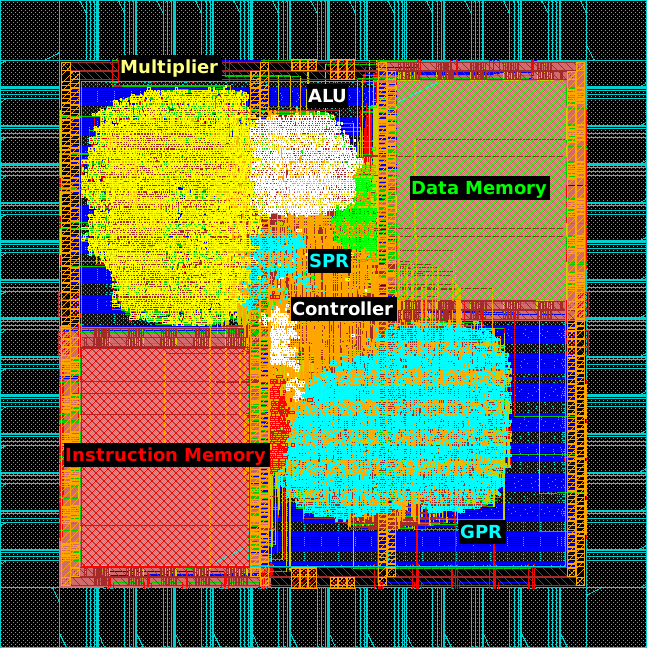
\includegraphics[width=\linewidth]{./figures/chip_colored}
  \caption{Area Distribution}
  \label{fig:chip_area}
\end{figure}

\begin{table}[htbp]
 \caption{Area distribution}
 \label{tab:area_dist}
 \centering\begin{tabular}{|l|r|r|r|r|r|} \hline
Name & Area [GE] & Cells & Area [$\mu m^2$] & $A/A_{tot}$ & Core Area \\ \hline
chip & 89174 & 15742 	& $1'607'457$ & 100.0 \% & - \\ \hline
-- pads and bondings 	& - &-&$771'501$ & - & - \\ \hline
-- top & 88592 & 15601 	& $830'497$ & 99.3 \% & 68.7 \%  \\ \hline
--- cpu & 44393 & 15218 & $416'160$ & 49.8 \% & 34.4 \%  \\ \hline
----- alu   & 5717 & 2283  	& $53'597$ & 6.4 \% & 4.4 \%\\ \hline
----- controller  & 482 & 273  	& $4'515$ & 0.6 \% & 0.4  \%\\ \hline
----- mult & 16930 & 6192 	& $158'709$ & 19.0 \% & 13.1 \% \\ \hline
----- registers& 13797 & 4037  	& $129'341$ & 15.5 \% & 10.7 \% \\ \hline
----- sp registers & 1133 & 267 & $10'621$ & 1.3 \% & 0.9 \% \\ \hline
--- instruction memory&21753& 58& $203'929$ & 24.4 \% & 16.9 \% \\ \hline
--- data memory  & 22260  & 257 & $208'676$ & 25.0 \% & 17.3 \% \\ \hline
 \end{tabular}
\end{table}
\newpage
\section{Timing}
As we have seen in chapter \ref{sec:pipe} - Pipelining is optimally used if the longest path of all pipeline stages are balanced. In table \ref{tab:longest_paths} there are listed all longest paths of the according four pipeline stages IF, ID, EX, WB and the two multiplier stages, a more detailled timinig diagram is shown in Figure \ref{fig:timing} where all paths between the pipeline stages is illustrated in an abstract way. The main stages are quite the same, but the Instruction Fetch stage is obviously quite shorter than the others. Combining with ID or WB seems not to be a feasible solution because they are already long enough and retiming could balance it but would lead to a less understandable design. 
\begin{table}[htbp]
 \caption{Longest Paths}
 \label{tab:longest_paths}
 \centering\begin{tabular}{|l|r|r|r|} \hline
\textbf{Pipeline Stage} & \textbf{$t_{pd}$} & \textbf{$t_{su}$} & \textbf{$\Sigma{t}$} \\ \hline
Instruction Fetch & 2.28 ns & 0.12 ns & 2.40 ns \\ \hline
Instruction Decode & 2.54 ns & 0.19 ns & 2.73 ns \\ \hline
Execute & 2.55 ns & 0.19 ns & 2.74 ns \\ \hline
- Execute ALU & 2.55 ns & 0.19 ns & 2.74 ns \\ \hline
- Execute Mult & 2.44 ns & 0.17 ns & 2.61 ns  \\ \hline
- Execute Mult 2 & 2.43 ns & 0.13 ns & 2.56 ns \\ \hline
Write Back & 2.55 ns & 0.19 ns & 2.74 ns \\ \hline \hline
Maximum & 2.59 ns & & 2.74 ns \\ \hline
Mean & 2.48 ns & & 2.63 ns\\ \hline
Standard Deviation & 0.15 ns & & 0.13 ns \\ \hline
 \end{tabular}
\end{table}

\begin{landscape}
\begin{figure}[htbp]
  \centering
  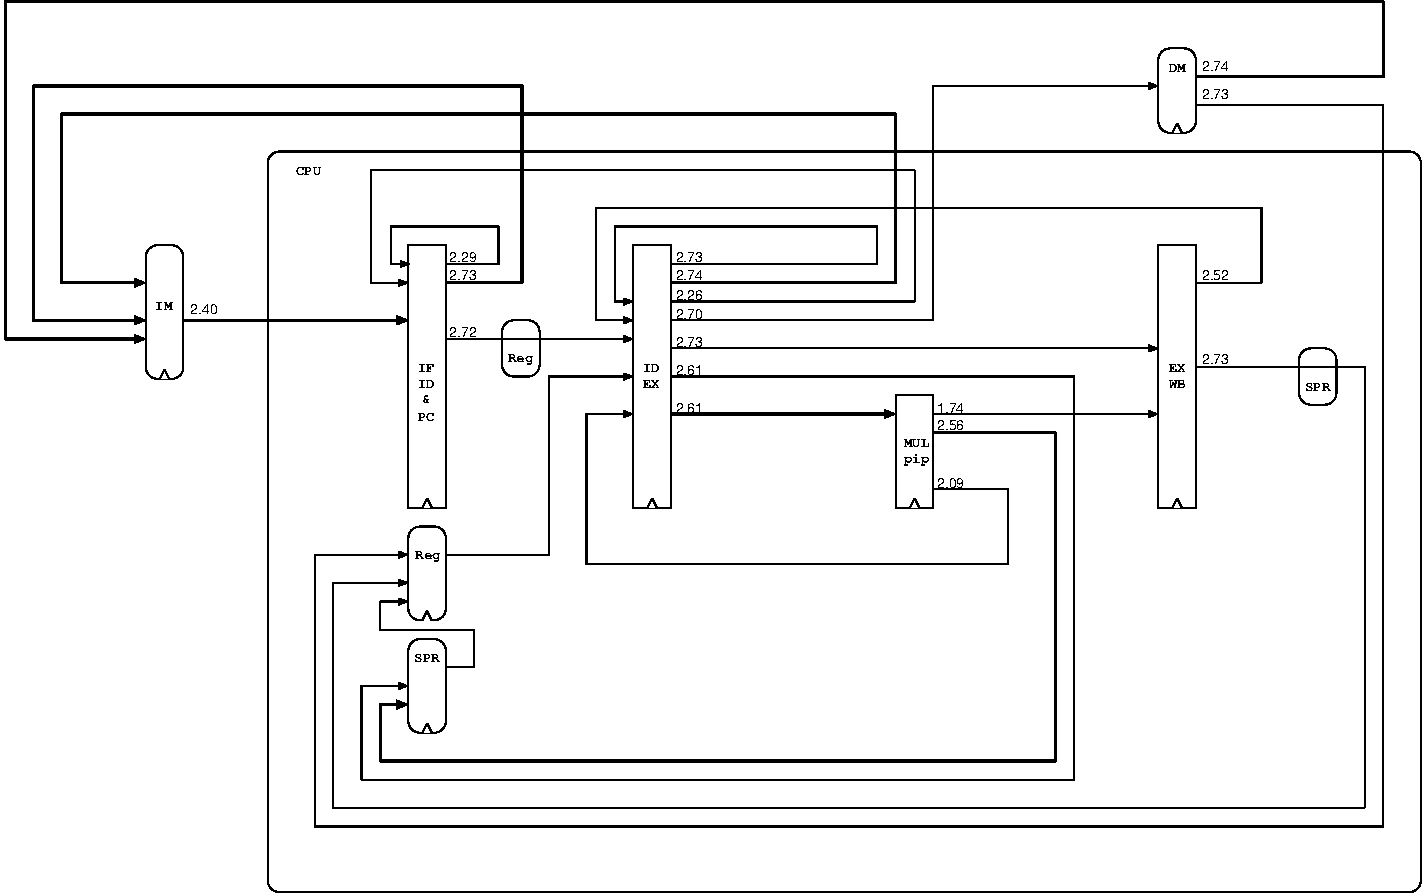
\includegraphics[width=\linewidth]{./figures/timing_diagram}
  \caption{Timing Diagram}
  \label{fig:timing}
\end{figure}

\end{landscape}

\section{Power}
Stichwort IR Drop, electromigration
\begin{table}[htbp]
 \caption{Power}
 \label{tab:power}
 \centering\begin{tabular}{|l|r|r|r||r||r|c|} \hline
program & $P_{SETUP}$ & $P_{RUN}$ & $P_{OUT}$ & $V_{cc_{min}}$ & $I_{max}$ & $\frac{J}{J_{max}}$ \\ \hline
full\_coverage.S & 53.9 $mW$ & 166.7 $mW$ & 64.8 $mW$ & 1.7943 $V$ & 6.97 $mA$ & 22 \% \\ \hline
matrixMul.c & 41.6 $mW$ & 161.2 $mW$ & - & 1.7905 $V$ & 11.42 $mA$ & 35 \% \\ \hline
matrixAdd.c & 43.5 $mW$ & 162.2 $mW$ & - & 1.7900 $V$ & 12.02 $mA$ & 37 \% \\ \hline
fibonacci.c & 44.5 $mW$ & 171.5 $mW$ & - & 1.7902 $V$ & 11.83 $mA$ & 35 \% \\ \hline \hline
mean/min/max & 45.9 $mW$ & 165.4 $mW$ & 64.8 $mW$ & 1.7900 $V$ & 12.02 $mA$ & 37 \%  \\ \hline
 \end{tabular}
\end{table}


\section{Floorplaning}
The floorplan is illustrated in Figure \ref{fig:chip_area}.
